\paragraph{Modules}
The software will provide `modules' which each contain some vocabulary to be learned.
The module order will correspond with the order in which the vocabulary should
be learned during semester. Each module will contain three challenges:
\begin{enumerate}
	\item Vocabulary List - Displays a list of vocabulary for the user to scan
		over and memorise.
	\item Test - Test the user on their knowledge of all the vocabulary for
		that module.
	\item Review - Test the user on a random selection of vocabulary from that
		module and all previous modules.
\end{enumerate}

It is expected that three modules will be completed each week for the six week
duration of the project for a total of 18 modules. It will not be explicitly
mentioned to the students that they should complete three modules per week,
however some might work this out on their own accord.
The key reason for this is that by allowing autonomy, students do not feel 
pressured into completing the challenges and believe they are completing them 
by their own will - an important defining feature of `play' vs `work'\cite{sebastian_deterding_meaningful_2011}.

\paragraph{Challenges}
For each module, three challenges will be available as discussed in the section
above. However, the availability of the challenges will be dependant upon the
group the user is assigned to. Group A (control) will have access to all
challenges at all levels from the beginning of the project. Group B will have
access only to the challenges on the first module. By completing the \textit{Test}
challenge, the following level will be unlocked. This game mechanic instills
a sense of \textit{achievement} in the student, encouraging them to unlock further
challenges \cite{gabe_zichermann_fun_2010}.


\begin{figure}[H]
	\centering
		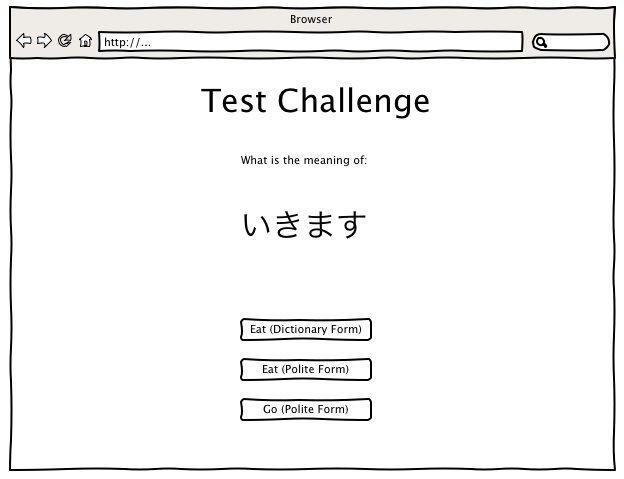
\includegraphics[width=10cm]{./screens/challenge.jpg}\\
		\caption{Mockup of a screen showing a challenge in progress}
\end{figure}

\paragraph{Points}
(Applies to Group B only)

Completing some challenges will earn the user points. The number of points earned is
dependant upon the module to which the challenge belongs, where increasing modules
result in more points earned. The Vocabulary List challenge will earn no points,
and is only available for the purpose of memorising for the Test challenge. The
Test challenge will earn the user points when it is completed the first time only
for each module. However completing the Test challenge will unlock the Review
challenge which the user can complete as many times as they wish, each time earning
points. Once the Review challenge has been completed successfully, the user must
wait 4 hours before attempting again to avoid misuse.


\begin{figure}[H]
	\centering
		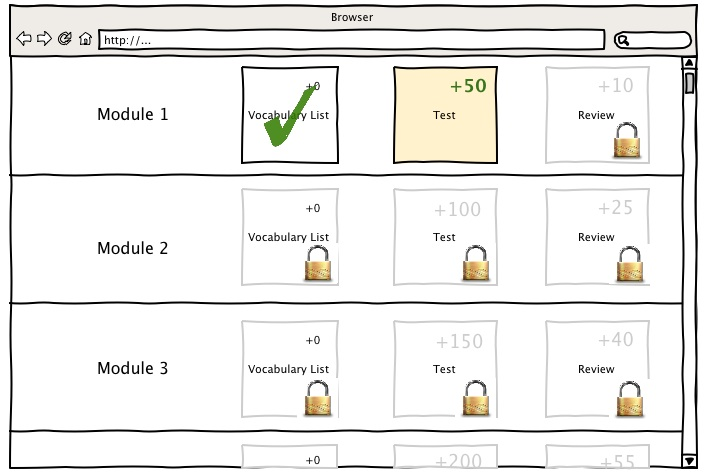
\includegraphics[width=10cm]{./screens/modules.jpg}\\
		\caption{Mockup of the list of available modules with associated challenges}
\end{figure}

\paragraph{Leaderboard}
(Applies to Group B only)
The leaderboard displays other users with a similar number of points and shows
the user how they can overtake the user above them by completing another
challenge. All users are given a ranking within the system based on their
number of points, however users can only see the ranking of other users within
three ranks of their own. This avoids leaving users feeling disappointed with
their current position and instead presents to them an achievable goal - that is to
overtake the user above them in ranking \cite{gabe_zichermann_fun_2010}.

\begin{figure}[H]
	\centering
		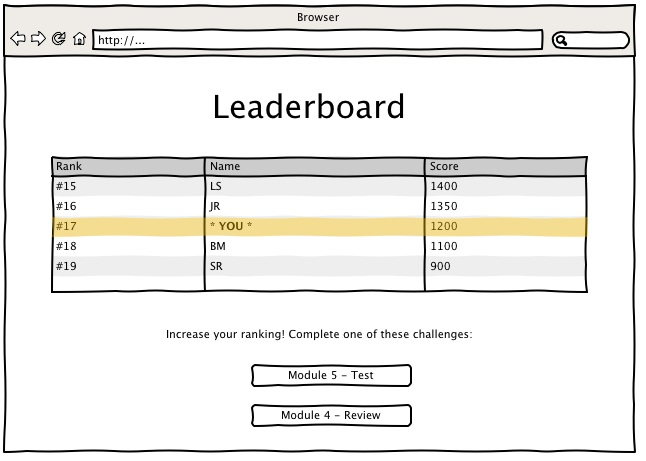
\includegraphics[width=10cm]{./screens/leaderboard.jpg}\\
		\caption{Mockup of the leaderboard showing similarly ranked users}
\end{figure}
